\documentclass{article}


%package
% ============================================ %
\usepackage{geometry}
\usepackage{authblk}
\usepackage{multicol}
\usepackage{blindtext}
\usepackage{titlesec}
\usepackage{xcolor}
\usepackage{array}
\usepackage[utf8]{inputenc}
\usepackage{graphicx}
\usepackage[font=small,labelfont=bf]{caption}
% ============================================ %


% formatting
% ============================================ %
\titleformat{\section}{\large\bfseries}{\thesection}{1em}{}
\titleformat{\subsection}{\small\bfseries}{\thesubsection}{0.7em}{}
\renewcommand\Authfont{\fontsize{12}{14.4}\selectfont}
\graphicspath{ {img/} }

 \geometry{
 a4paper,
 total={170mm,257mm},
 left=15mm,
 right=15mm,
 top=1mm,
 bottom=20mm
 }
% ============================================ %

% title
% ============================================ %
\title{\textbf{Haters Gonna Hate}\\
  \large Check-in Report 3\\}


\author[1]{\large Aviral Chawla}
\author[2]{\large Daniel Orem}
\author[3]{\large Jay Hwasung Jung}
\author[4]{\large Shunsuke Miyazato}

\affil[1]{\footnotesize Complex Systems and Data Science (CSDS) M.S., University of Vermont}
\affil[2]{\footnotesize Chemistry (CHEM) B.S., University of Vermont}
\affil[3]{\footnotesize Computer Science (CS) B.S., University of Vermont}
\affil[4]{\footnotesize Data Science (DS) B.S., University of Vermont}
\date{ \small Nov 27, 2022}
% ============================================ %

% documents
% ============================================ %
\begin{document}
\maketitle
\vspace{-10mm}
% abstract
\begin{abstract}
Social media is widely used across continents, generations, and social groups. Due to the accessibility and anonymity of social media, hate speech, an abusive or threatening statement showing prejudice and hate, has become a new social phenomenon and has gotten public attention. In previous research, there has been an effort to understand the behavior of such hateful speech using Natural Language Processing and Networks, and social media platforms have hate-speech detection models based on such research. Although research provides an effective method to detect hateful speech, research understanding its behavior still needs to be completed. This project aims to provide the framework for social media platforms to conduct an early intervention in hate speech using network behavior of content instead of relying on language models for classification. 
\end{abstract}

\begin{multicols}{2}
\section{Activities}
    \subsection{Planned Activities}
      
    \hspace{5mm}For week 03 and week 04, our goal was to polish classification process get datasets, and assess model accuracy and start building a network. 
    \subsection{Accomplished Activities}
    \hspace{5mm} For week 03 and week 04, we tried to clean our datasets, and save it as a .db format, so we can retrieve datasets anytime we want. Also, last week, we did some machine learning model testings. Moreover, we found the API called Google Perspective which evaluates the score of texts in requested categories such as Toxisity, etc...
    
    Below is the scores listed using Google Perspective API. These scores indicate probabilities that the given texts are classified as a category such as Toxicity, Insult, or Treat.
    
    \vspace{2mm}
    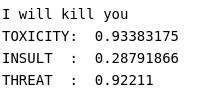
\includegraphics[scale=0.49]{image.png}
    \vspace{-3mm}

    \captionof{figure}{\textbf{Google Perspective API scores of three categories}}
    \vspace{2mm}
    \hspace{5mm}We are expecting to compare this model with machine learning models we built and compare the effectiveness of them.
\section{Challenges}
    \subsection{Open Challenges and Questions}
    \hspace{5mm}Due to the time constraints during the Thanksgiving, it was hard to communicate with teammates. Also, getting an "increasing quota" for Google Perspective API takes long. Originally, this API can request 60 times/minutes, but it will take us overnight to analyze all datasets we have; if there is an update in our model, we cannot help re-running the evaluation and classification.
    
    \subsection{Major Changes}
        \hspace{5mm}Networks will be built next week. 
\section{Timeline and Roles}
    \subsection{Timeline}
        \begin{tabular}{m{3.8em} | m{19em}} 
        \hline
        Time & Task \\ [0.5ex] 
        \hline\hline
        \small Week 01 & Literature review finish project proposal \\ 
        \hline
        \small Week 02 & Extract data and work on cleaning and organizing it \\
        \hline
        \small Week 03 & Polish classification process and get a final model-tagged data to work with \\
        \hline
        \small Week 04 & Assess model accuracy and start building the network \\
        \hline
        \small Week 05 & Network analysis and visualization \\
        \hline
        \small Week 06 & Compile results and prepare final report \\
        \end{tabular}
    \subsection{Roles}
        \begin{tabular}{m{7.8em} | m{15em}} 
        \hline
        Name & Tasks \\ [0.5ex] 
        \hline\hline
        \small Aviral Chawla & Build Hate speech Network based on the classification of our models. \\ 
        \hline
        \small Daniel Orem & Analyze classified data in-depth\\
        \hline
        \small Jay Hwasung Jung & Build Hate Speech network and housekeep models.  \\
        \hline
        \small Shunsuke Miyazato & Analyze classified data in-depth\\
        \end{tabular}
\end{multicols}

\end{document}